%===========================================================================
\section{Uncertainty quantification}
\label{section:uncertainty}
%----------------------------------------------------------------------------------
%----------------------------------QUANTIF-----------------------------------------
%----------------------------------------------------------------------------------
\subsection{Used Tool : Uncertainty treatment library OpenTURNS}
OpenTURNS (Open source initiative to Treat Uncertainties, Risks'N Statistics) \cite{bib11} is an open source C++ Library for uncertainty treatment used through python scripts. It is co-developed since 2005 by EADS IW, EDF R\&D and PHIMECA Engineering. Various statistical methods are implemented in this library and allow to follow the uncertainty study steps \cite{bib18} represented in Figure \ref{fig:uncertainty_diagram}.
\begin{figure}[h!]
    \centering
    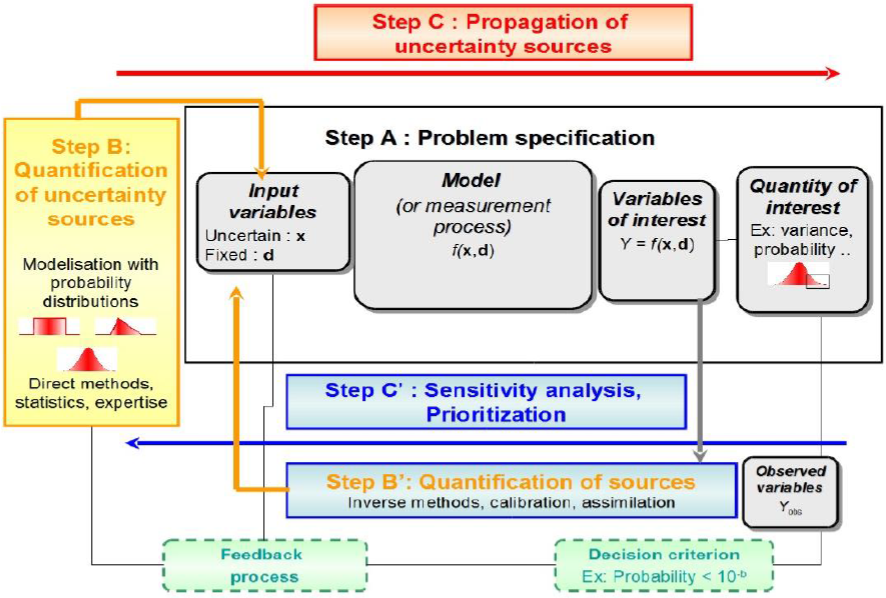
\includegraphics[trim={0 0 0 0},clip,scale=0.5]{Images/Uncertainty_diagram}
    \vspace{-0.2cm}
    \caption{Steps for an uncertainty study}
    \label{fig:uncertainty_diagram}
    \vspace{-0.5cm}
\end{figure}

%----------------------------------------------------------------------------------
\subsection{Uncertainty sources quantification}
\label{subsection:quantification}
The goal here is to define variation intervals and probability density functions (PDF) for each uncertain parameters. We remind that, for a random variable X defined on an interval $[a,b]$, a PDF $f(x)$ is defined as follows :
\begin{equation}
\mathbb{P}(X \in [a,b])=\int_a^b f(x)dx
\end{equation}

For all the variables from 2 to 8 defined in Table \ref{tab_var_PDF}, variation intervals were found in literature, without further information about their probabilities. Consequently, using the principle of maximum entropy \cite{bib19}, uniform probability density functions are chosen for those variables. 

For the experimental channel case, only one mean diameter measure is available and is subject to measurements errors. The errors interval is considered as a variation interval and a uniform PDF is applied for the mean diameter on its measurement interval. For the real bifurcation case, several samples of sediments are extracted in different sections of the river. Different values of the mean diameter are possible. In order to take all of them into consideration, a PDF that corresponds to the sample is selected and validated via the QQ-Plot method \cite{bib11}.

%The summarized variables and their probability density functions are presented in Table \ref{tab_var_PDF}.
%\begin{table}[!h]
%\centering
%\begin{tabular}{|C{1.5cm}|C{3cm}|C{3cm}|}
%\hline
%{Variable} &{Definition} & {PDF}\\
%\hline $d$ & Sediments mean diameter & Uniform[1,2] \\
%\hline $A_{g}$ & Green's transport coefficient & Uniform[5,15]\\
%\hline $\lambda$ & Porosity & Uniform[0.25,0.4]\\
%\hline $\alpha_S$ & Skin friction coefficient & Uniform[1.0,6.6]\\
%\hline $\Phi_S$ & Angle of repose of the sediments (Slope effect on transport direction)  & Uniform[30,80] \\
%\hline $\beta_2$ & Deviation parameter (Slope effect on transport amplitude) & Uniform[0.1,5.0] \\
%\hline
%\end{tabular}
%\caption{Uncertain parameters and their PDFs}
%\label{tab_var_PDF}
%\vspace{-0.5cm}
%\end{table}
